\htwo{WebUntis}
\sectionauthor{Mersed Kečo}

\hthree{Einleitung}

WebUntis ist der zentrale Ort, wo die Planung für eine Schule vorgenommen werden kann. Entscheidungen sind mithilfe von WebUntis leichter zu treffen und Informationen sind immer direkt griffbereit, nicht nur für Lehrer und die Administration der Schule, sondern auch für Schüler und deren Eltern. Da das Schulzentrum Ungargasse WebUntis jetzt schon einige Zeit verwendet, bietet es eine solide Grundlage für die Informationsgewinn – und Verarbeitung. Damit das Zelia-Team überhaupt eine Möglichkeit besitzt, auf Stundenpläne von Klassen und auf bestimmte Räume zugreifen zu können, benötigt es eine REST-API. In unserem Fall gibt es einen bereits bestehende Node.Js-Wrapper der WebUntis-API mit einer doch sehr weiterhelfenden Dokumentation zu den darin bestehenden Methoden und den zu verwendenden Parametern. Dieser wird aber nicht direkt von WebUntis bereitgestellt, sondern von einer kleinen Community auf GitHub. \cite{WebUntisWrapper}

\begin{figure}[h]
    \centering
    
\includegraphics{media/WebUntis/WebUntisLogo.png}
    \caption{WebUntis Logo\cite{WebUntisLogo}}
\end{figure}

\hfour{Geschichte}

Untis wurde am 7.Jänner 1970 von den beiden Programmierern, Bernhard Gruber und Heinz Petters gegründet. Der Hintergrund, warum sich die beiden vor allem für einen Online-Stundenplan entschieden haben in einer Zeit, wo noch nicht einmal der Gedanke eines Online-Klassenbuches im Raum stand, ist nicht ersichtlich. Dennoch prägt ihre bahnbrechende Entwicklung nicht nur österreichische, sondern auch über 26.000 Schulen international mit einem sehr großen Supportnetz. \cite{Untis}

\hthree{Implementierung}

Um den Wrapper überhaupt verwenden zu können, benötigt man zuerst das WebUntis-Package, welches man sich wie folgt runterlädt und installiert:

\emph{npm i webuntis}

Durch den Wrapper hat man die Möglichkeit auf nicht nur den Stundenplan und gewisse Informationen zu diesem zu gewinnen, sondern auch zum Beispiel Informationen zur besuchten Fachabteilung oder das Anzeigen von Hausübungen. In diesem Fall benötigen wir aber nur folgende Methoden, die teilweise mit anderen Methoden verwendet werden, um auf unser Wunschergebnis zu kommen:


\typescript{code/WebUntis/constructor.ts}{Konstruktor von der WebUntis API}

Der Konstruktor muss so verwenden werden, da man sonst nicht auf das WebUntis-Objekt zugreifen kann. Bei Zelia wird es genauso verwendet, der einzige Unterschied ist aber hierbei, dass unsere Variablen und die dazu entsprechenden Werte in einem .env-File abgespeichert sind, damit erstens, die Daten alle gesammelt an einer Stelle liegen und zweitens, da somit ein wenig Sicherheit reingebracht werden kann.

\typescript{code/WebUntis/.env.ts}{.env-Datei von Zelia}

getRooms wird verwendet, um alle Räume für ein Schulgebäude herauszufinden.

\typescript{code/WebUntis/getRooms.ts}{getRooms Methode}

Dies ist nur ein kleiner Ausschnitt der gesamten Räume des SZU:

\begin{figure}[h]
    \centering
    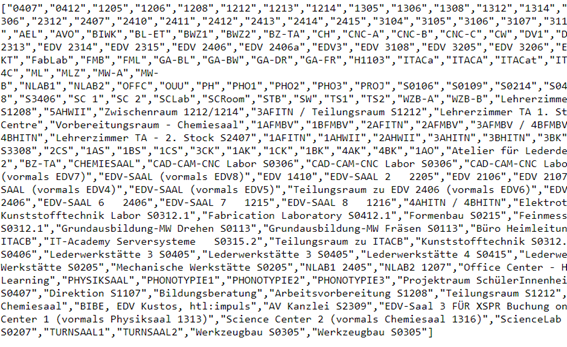
\includegraphics{media/WebUntis/getRoomsAusgabe.png}
    \caption{getRooms Ausgabe Zelia}
\end{figure}

Mithilfe der Methode getTimetableFor und den mitzugebenden Parametern können wir uns den Stundeplan für einen speziellen Typen anzeigen lassen.

\typescript{code/WebUntis/getTimetableFor.ts}{getTimetableFor Beschreibung}

Der WebUntisElementType wird als Wert übergeben und je nachdem, welcher Wert das ist, so wird der Stundenplan ausgegeben. 

\begin{figure}[h]
    \centering
    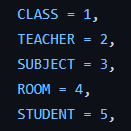
\includegraphics{media/WebUntis/WebUntisElementType.png}
    \caption{WebUntisElementType}
\end{figure}


In der Ausgabe können wir also alle wichtigen Parameter sehen, sei es das Fach, die Klasse die momentan unterrichtet wird oder aber auch der Lehrer, der die Stunde abhält.

\typescript{code/WebUntis/getTimetableForAusgabe.ts}{getTimetableFor Zelia}

Die Methode "getTimeGrid" wird verwendet, um die Struktur des Stundeplans anzuzeigen. Mit der Struktur sind die Unterrichtsstunden, deren Anfangs – und Endzeiten gemeint.

\typescript{code/WebUntis/getTimegrid.ts}{getTimegrid Methode}

Das Ergebnis sieht bei Zelia wie folgt aus:

\typescript{code/WebUntis/getTimegridAusgabe.ts}{getTimeGrid Zelia}

\hfour{Probleme}

Mithilfe der API ist zwar einiges möglich, dennoch sind uns in dem Anwendungsfall Zelia einige "Probleme" aufgefallen, die abgefangen beziehungsweise ausgebessert werden mussten.

Das allererste Problem ist, dass gewisse Räume mit mehreren Namen beziehungsweise mehreren IDs eingetragen sind und anfänglich die Frage im Raum stand, nach welchen Kriterien man den Klassenraum auffindet. Bei Zelia ist man sich aber im Endeffekt einig geworden, nach der ID des Raumes zu suchen.

\typescript{code/WebUntis/getIDByRoomNumber.ts}{Raum über ID zurückbekommen}


Die Methode bekommt einen Wert des Typen "RoomNumber" übergeben. Gleichzeitig beschaffen wir uns mit der Methode getRoomList() alle eingetragenen Klassen und gehen in einer for-Schleife durch jedes Element durch. Die Vorgehensweise scheint zwar unprofessionell, doch während der Implementierung ist aufgefallen, dass der vollständige Klassenname nicht immer im Longname oder im Shortname abgespeichert, sondern eher rein zufällig in einem der beiden Parametern beinhaltet ist. Deswegen prüfen wir auf Nummer sicher beide Parameter ab und geben bei einer Übereinstimmung die dazu vorhandene Raum-ID mit, diese ist einzigartig dennoch können wie schon zuvor gesagt, mehrere IDs auf einen Raum zeigen, was in dem Fall kein allzu großes Problem darstellt.

Des Weiteren gab es das Problem, das WebUntis einen Token eingebaut hat, welcher nach einer gewissen Zeit abläuft und die momentane Sitzung als "ungültig" deklariert.In diesem Fall können wir mit der Methode validateSession() abprüfen, ob der Token zum Zeitpunkt der Abfrage schon abgelaufen oder noch gültig ist. 

\typescript{code/WebUntis/validateSession.ts}{Abfrage eines "gültigen" Tokens}


Falls der Token zum Zeitpunkt der Abfrage ungültig ist, wird die Variable valid auf "false" gesetzt und springt nach der if-Abfrage in den else-Zweig. Dort wird automatisch eine Neuanmeldung mit den Informationen des Benutzers getätigt und es wird erneut versucht, die gewünschte Methode auszuführen.

\pagebreak

Während dem Exception-Handling ist uns folgender Fehler seitens WebUntis aufgefallen:

\typescript{code/WebUntis/ExceptionHandling.ts}{ExceptionHandling}

Wenn der WebUntis-Server kein Ergebnis auf eine Anfrage zurückgesendet, schickt dieser eine Exception-Message, die wir in diesem Fall abfangen. Leider ist aber die Nachricht falsch geschrieben und der Fehler ist nicht direkt ersichtlich, außer man liest sehr genau. Dieser Fehler wird aber mit dem Code in der nahestehenden Abbildung abgefangen und macht weitergehend keine Probleme im Code.